\section{Ring Counting}
\label{sec:ring_counting}
The ring counting algorithms in APFIT have never been tuned for high energy events.  As it turns out, APFIT finds phantom rings in many high energy electromagnetic showers, as in Figure \ref{fig:phantom_ring.png}.  Because of this, the efficiency of the 1-ring cut for this analysis drops off very sharply around 10 GeV if no adjustment is made, as shown in Figure \ref{fig:eff_oldrings}. 
\begin{figure}
	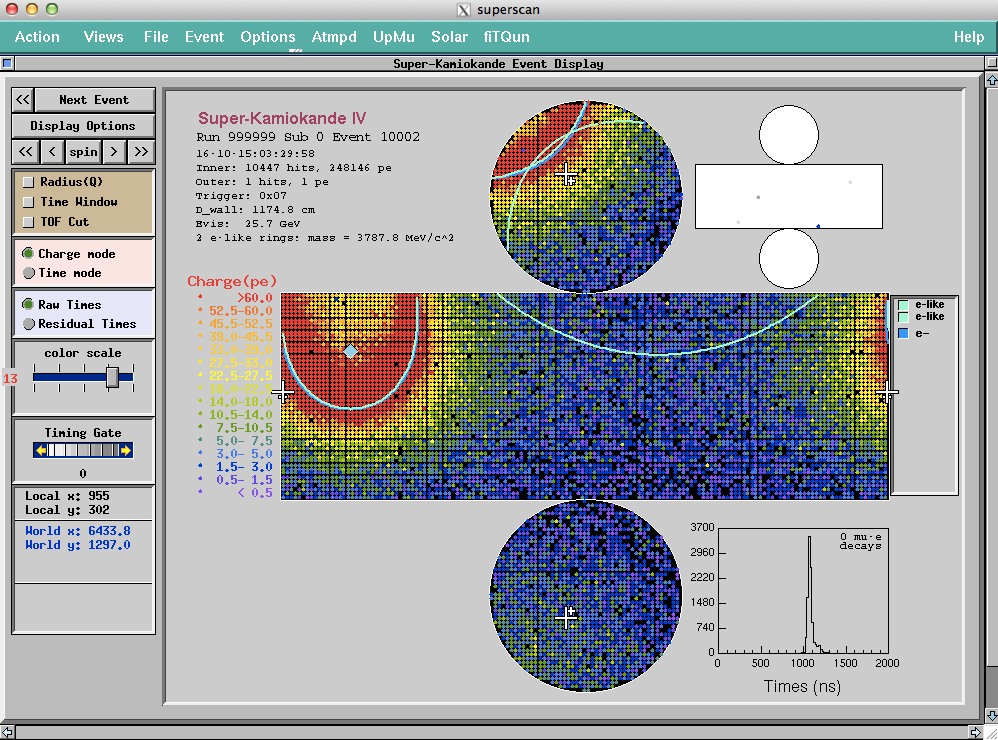
\includegraphics[width=0.6\textwidth]{figures/display_phantom.png}
	\caption{Example of a phantom ring found by APFIT.  This is a single electron at 28 GeV.  APFIT correctly finds the ring corresponding to the electron, but also finds an additional phantom ring}
	\label{fig:phantom_ring.png}
\end{figure}

\begin{figure}
	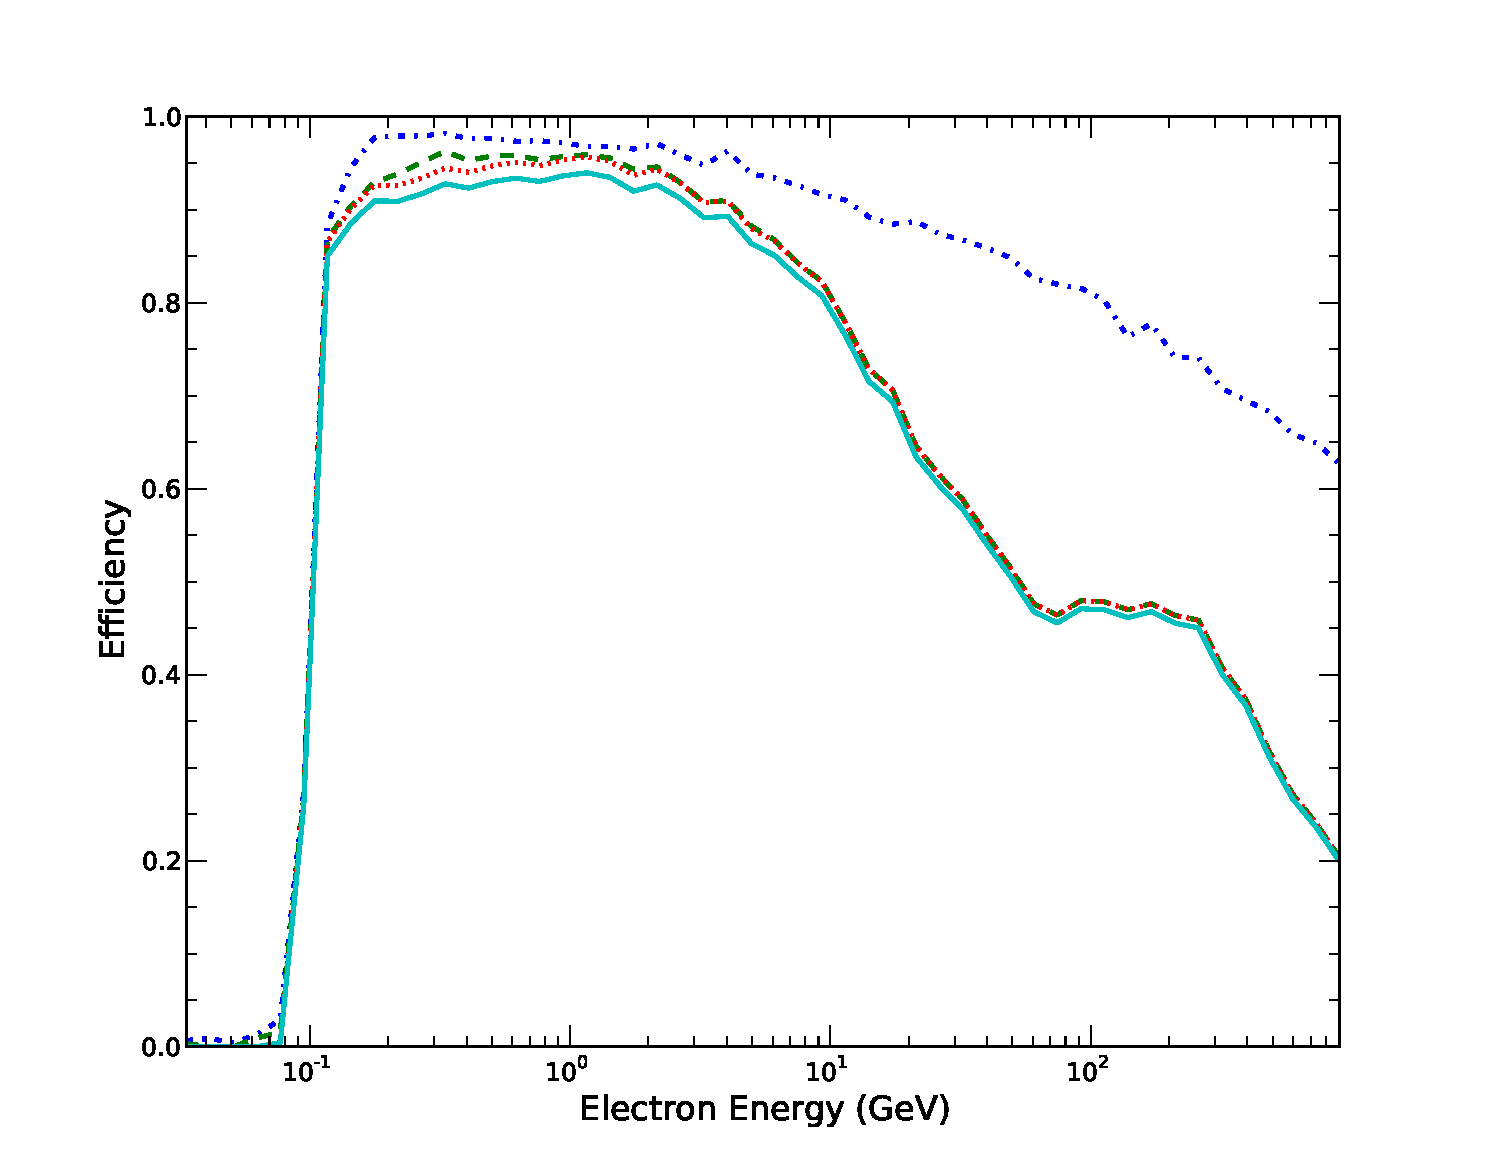
\includegraphics[width=0.6\textwidth]{figures/efficiency_30MeV_1TeV_old1ring.pdf}
	\caption{Effeciency of the selection and analysis cuts as a function of energy, with no ring counting adjustment.  Color scheme is the same as in Figure \ref{fig:eff}.  Note the sharp drop in the efficiency of the 1-ring cut (dashed green).}
	\label{fig:eff_oldrings}
\end{figure}

These phantom rings are caused by fluctuations in the light patterns of high energy events.  Because there is a large amount of light in a high energy event, these statistical fluctuations can trick APFIT into thinking it sees a low energy ring in addition.  To fix this pathology, a test variable is constructed to merge rings which could reasonably be caused by statistical fluctuations:
\begin{equation}
	\alpha^2_{i_\textrm{ring}}=\frac{1}{N_{\textrm{PMT},\theta<70^\circ}} \sum \limits_{j_{\textrm{PMT}\theta<70^\circ}} \frac{Q\textrm{Dev}_{i_\textrm{ring},j_\textrm{PMT}}^2}{Q\textrm{Dev}_{i_\textrm{MER},j_\textrm{PMT}}}
	\label{eq:alpha}
\end{equation}
where $N_{\textrm{PMT}\theta<70^\circ}$ is the number of PMT's within $70^\circ$ of the direction of the ring, $i_\textrm{MER}$ is the index of the most energetic ring, and $Q\textrm{Dev}_{i,j}$ is the devided charge of the j$^\textrm{th}$ PMT assigned to the i$^\textrm{th}$ ring, defined as:
\begin{equation}
 	Q\textrm{Dev}_{i,j}=Q_j^\textrm{measured}\frac{Q_{i,j}^\textrm{expected}}{\sum \limits_k Q_{k,j}^\textrm{expected}}
	\label{eq:qdev}
\end{equation}		
where $Q_{i,j}^\textrm{expected}$ is the charge expected in the j$^\textrm{th}$ PMT due to the i$^\textrm{th}$ ring and $Q_j^\textrm{measured}$ is the charge measured in the j$^\textrm{th}$ PMT.   $Q\textrm{Dev}_{i,j}$ is stored in the common block array APPEDEV in APFIT.  In order to fill APPEDEV with usable values, sprngsep(2,1,1,3) is run.  For rings which are not the most energetic ring, $\alpha$ is calculated, and the ring is merged into the most energetic ring if $\alpha<0.6$.  Figure \ref{fig:apdev} shows the distribution of values of $\alpha$ for real and fake rings in the signal electromagnetic shower and background atmospheric neutrino MC.  Since, the 1-ring cut efficiency is only problematic at high energies, this merging technique is only applied to events with E$_\textrm{vis}>$1.33 GeV.  With merging, the efficiency improves from that seen in Figure \ref{fig:eff_oldrings} to that seen in Figure \ref{fig:eff}, with minimal increase of the atmospheric background.  



\begin{figure}
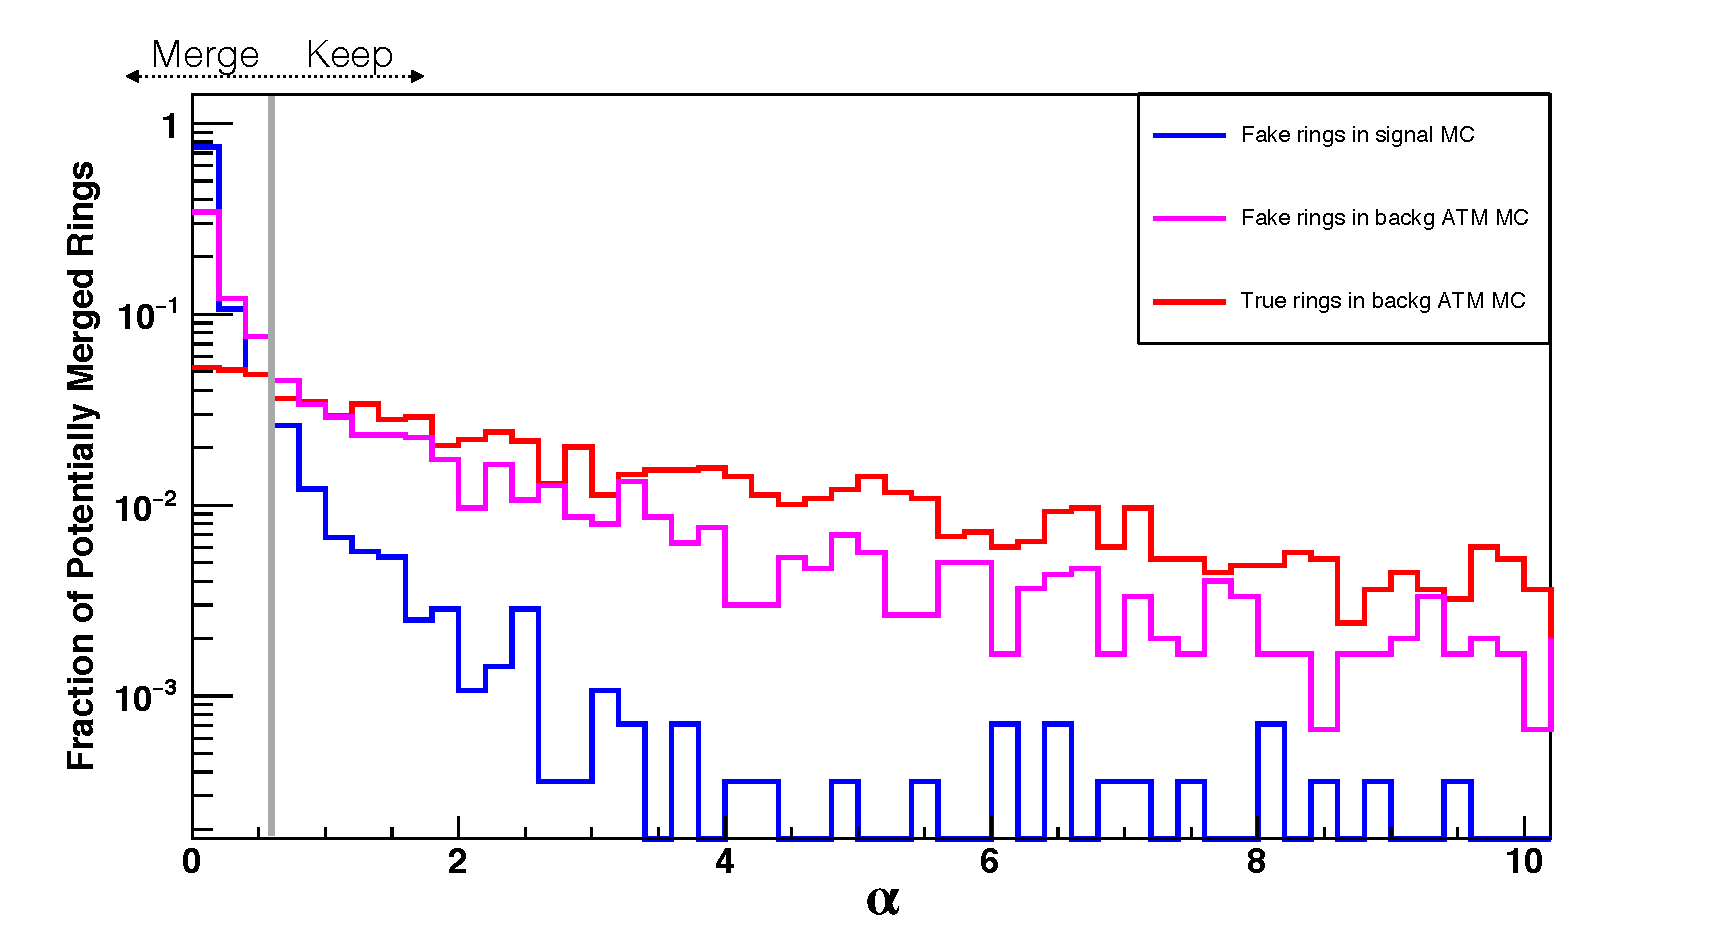
\includegraphics[width=0.6\textwidth]{figures/apdev.pdf}
\caption{Test variable for merging rings in high energy events.  If $\alpha>0.6$, the ring is merged into the most energetic ring.}
\label{fig:apdev}
\end{figure}